\begin{example}[One peel commit, then two centroid batches]
\label{ex:algorithm-peel-centroids-20260918}
Let $\ResidualPositions=[15]$, $\DegreeCutoff=9$, and let the current
residual forest have edge set
\[
 E=\{\{1,i\}:2\le i\le9\}
   \cup\{\{1,10\},\{10,11\},\{11,12\},
          \{1,13\},\{13,14\},\{14,15\}\}.
\]
Vertex $1$ has degree $10$; every other vertex has degree at most $2$.
Suppose the reached screens are successful.  By
\AppLowDegreeScreenRef, $\ScreenRow{u}=\mathcal N_{\ResidualForest}(u)$
for $u\ne1$, whereas the row $\ScreenRow{1}$ need not be exact.
Nevertheless, \eqref{app:eq:claim-and-peel-set} gives
\begin{align*}
 \ClaimCount{1}
 &=\sum_{u\ne1}\mathbf1\{1\in\mathcal N_{\ResidualForest}(u)\}=10>9/2,\\
 \ClaimCount{v}
 &=|\mathcal N_{\ResidualForest}(v)\setminus\{1\}|
     +\mathbf1\{v\in\ScreenRow{1}\}
 \le2+1=3<9/2 \quad(v\ne1).
\end{align*}
Hence $\PeelSet=\{1\}$, regardless of the high-degree row's contents.
In \AlgoBlockRef{peel}, the sampler freezes this set and commits
vertex $1$ alone.  The residual
components are then
\[
 \{2\},\ldots,\{9\},\qquad
 10\text{--}11\text{--}12,\qquad 13\text{--}14\text{--}15.
\]
The next pass through \AlgoBlockRef{screen} uses the new history, before
the stopping test in \AlgoBlockRef{peel}.
Every residual degree is now at most $2$, so all its rows are exact.
Every incoming count is at most $2<9/2$, giving an empty peel set and
the exact terminal forest in \AlgoBlockRef{terminal}.
The successive batches of \AlgoBlockRef{centroid} are
\[
 B_1=\{2,\ldots,9,11,14\},\quad |B_1|=10,
 \qquad
 B_2=\{10,12,13,15\},\quad |B_2|=4.
\]
The eight isolates and the two path centers form $B_1$; deleting them
leaves the four singleton components in $B_2$.
Thus the example uses $1+2=3$ commit rounds.
This count excludes screen submissions and is not the total oracle depth.
\Cref{fig:algorithm-workflow-20260918} keeps the vertex positions fixed
throughout these steps.
\end{example}

\begin{figure}[H]
 \centering
 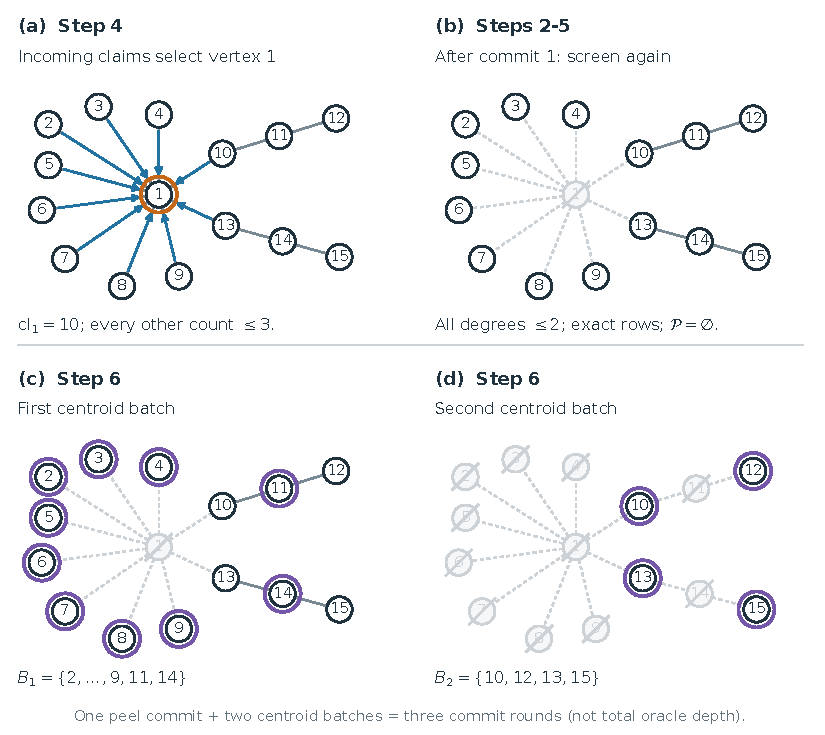
\includegraphics[width=\linewidth]{figures/algorithm_examples_2026-09-18/output/pdf/workflow_2026-09-18.pdf}
 \caption{The successful-screen path of
 \cref{ex:algorithm-peel-centroids-20260918}, with $N=15$ and $d=9$.
 Orange and violet rings denote the next peel or centroid commit;
 pale crossed vertices are already committed. The fills here are
 neutral, not random colors. The step labels refer to
 Algorithm~\ref{app:alg:complete-sampler}. A fresh screen separates (a) from (b);
 the terminal forest then needs no further discovery. All vertices
 remain individually visible.}
 \label{fig:algorithm-workflow-20260918}
\end{figure}
